\pdfoutput=1
\documentclass[a4paper,pdflatex,ja=standard]{bxjsarticle}

% ---Setting about the geometry of the document----
% \usepackage{a4wide}
% \pagestyle{empty}

% ---Physics and Math Packages---
\usepackage{amssymb,amsfonts,amsthm,mathtools}
\usepackage{physics,braket,bm}

% ---underline---
\usepackage{ulem}

% --- sorround the texts or equations
% \usepackage{fancybox,ascmac}

% ---settings of theorem environment---
% \usepackage{amsthm}
% \theoremstyle{definition}

% ---settings of proof environment---
% \renewcommand{\proofname}{\textbf{証明}}
% \renewcommand{\qedsymbol}{$\blacksquare$}

% ---Ignore the Warnings---
\usepackage{silence}
\WarningFilter{latexfont}{Some font shapes,Font shape}

% ---Insert the figure (If insert the `draft' at the option, the process becomes faster)---
\usepackage{graphicx}
% \usepackage{subcaption}

% ----Add a link to a text---
\usepackage{url}
\usepackage{xcolor,hyperref}
\hypersetup{colorlinks=true,citecolor=orange,linkcolor=blue,urlcolor=magenta}
\usepackage{bxcjkjatype}

% ---Tikz---
\usepackage{tikz,pgf,pgfplots,circuitikz}
\pgfplotsset{compat=1.15}
\usetikzlibrary{intersections,arrows.meta,angles,calc,3d,decorations.pathmorphing}

% ---Add the section number to the equation, figure, and table number---
\makeatletter
   \renewcommand{\theequation}{\thesection.\arabic{equation}}
   \@addtoreset{equation}{section}
   
   \renewcommand{\thefigure}{\thesection.\arabic{figure}}
   \@addtoreset{figure}{section}
   
   \renewcommand{\thetable}{\thesection.\arabic{table}}
   \@addtoreset{table}{section}
\makeatother

% ---enumerate---
\renewcommand{\labelenumi}{$(\arabic{enumi})$}
% \renewcommand{\labelenumii}{$(\arabic{enumii})$}

% ---Index---
% \usepackage{makeidx}
% \makeindex 

% ---Fonts---
\renewcommand{\familydefault}{\sfdefault}

% ---Title---
\title{京都大学 令和4年 物理学専攻 院試 解答例}
\author{ミヤネ}
\date{最終更新:\today}

\newcommand{\prb}[4]{
  \phantomsection
  \addcontentsline{toc}{subsection}{問題 #1-#2#3: #4}
  \section*{#1-#2#3\ :\  #4}
  \setcounter{subsection}{#2}
  \setcounter{equation}{0}
  \if{#3}{\empty} 
  \renewcommand{\theequation}{\thesubsection.\arabic{equation}}
  \else \renewcommand{\theequation}{\thesubsection#3.\arabic{equation}}
  \fi
}

\begin{document}

\maketitle

\tableofcontents
\clearpage

\section{パート1}
\prb{I}{1}{\empty}{量子力学}
\begin{enumerate}
  \item 
  運動エネルギーは$p^2/2m$なので
  \begin{equation}
    H_{B=0}
    =
    \frac{1}{2m}(p_{x}^2+p_{y}^2)
    +
    \frac{m\omega^2}{2}(x^2+y^2)
  \end{equation}
  である.

  \item 
  代入すれば
  \begin{align}
    \hat{H}_{B=0}
    &=
    -\frac{\hbar\omega}{4}
    \left\{ 
      (\hat{a}_{x}^\dagger-\hat{a}_{x})^2
      +
      (\hat{a}_{y}^\dagger-\hat{a}_{y})^2
    \right\}
    +
    \frac{\hbar\omega}{4}
    \left\{ 
      (\hat{a}_{x}^\dagger+\hat{a}_{x})^2
      +
      (\hat{a}_{y}^\dagger+\hat{a}_{y})^2
    \right\}
    \nonumber
    \\
    &=
    \frac{\hbar\omega}{2}\left\{ 
    \vphantom{\frac{1}{2}}
    \hat{a}_{x}^\dagger\hat{a}_{x}
    +
    \hat{a}_{x}\hat{a}_{x}^\dagger
    +
    \hat{a}_{y}^\dagger\hat{a}_{y}
    +
    \hat{a}_{y}\hat{a}_{y}^\dagger
    \right\}
    \nonumber
    \\
    &=
    \hbar\omega(\hat{a}_{x}^\dagger\hat{a}_{x}+\hat{a}_{y}^\dagger\hat{a}_{y}+1)
  \end{align}
  である.なお,交換関係$\left[ \hat{a},\hat{a}^\dagger \right]=1$を用いた.

  \item 
  $\hat{L}$とハミルトニアンの交換関係は
  \begin{align}
    \left[  
      \hat{H}_{B=0},\hat{L}
    \right]
    &=
    \left[  
      \frac{1}{2m}(\hat{p}_{x}^2+\hat{p}_{y}^2)
      +
      \frac{m\omega^2}{2}(\hat{x}^2+\hat{y}^2)
      ,
      \hat{x}\hat{p}_{y}-\hat{y}\hat{p}_{x}
    \right]
    \nonumber
    \\
    &=
    \frac{1}{2m}\left[ \hat{p}_{x}^2,\hat{x}\hat{p}_{y} \right]
    +
    \frac{1}{2m}\left[ \hat{p}_{y}^2,\hat{x}\hat{p}_{y} \right]
    -
    \frac{1}{2m}\left[ \hat{p}_{x}^2,\hat{y}\hat{p}_{x} \right]
    -
    \frac{1}{2m}\left[ \hat{p}_{y}^2,\hat{y}\hat{p}_{x} \right]
    \nonumber
    \\
    &\hspace{1cm}
    +
    \frac{m\omega^2}{2}\left[ \hat{x}^2,\hat{x}\hat{p}_{y} \right]
    +
    \frac{m\omega^2}{2}\left[ \hat{y}^2,\hat{x}\hat{p}_{y} \right]
    -
    \frac{m\omega^2}{2}\left[ \hat{x}^2,\hat{y}\hat{p}_{x} \right]
    -
    \frac{m\omega^2}{2}\left[ \hat{y}^2,\hat{y}\hat{p}_{x} \right]
    \label{HL}
  \end{align}
  だが,
  \begin{align}
    \left[ \hat{p}_{x}^2,\hat{x}\hat{p}_{y} \right]
    &=
    \left[ \hat{p}_{x}^2,\hat{x} \right]\hat{p}_{y}
    +
    \hat{x}\left[ \hat{p}_{x}^2,\hat{p}_{y} \right]
    =
    \hat{p}_{x}\left[ \hat{p}_{x},\hat{x} \right]\hat{p}_{y}
    +
    \left[ \hat{p}_{x},\hat{x} \right]\hat{p}_{x}\hat{p}_{y}
    =
    -2i\hbar\hat{p}_{x}\hat{p}_{y}
    \\
    \left[ \hat{p}_{y}^2,\hat{x}\hat{p}_{y} \right]
    &=
    \hat{x}\left[ \hat{p}_{y}^2,\hat{p}_{y} \right]
    +
    \left[ \hat{p}_{y}^2,\hat{x} \right]\hat{p}_{y}
    =
    0
    \\
    \left[ \hat{p}_{x}^2,\hat{y}\hat{p}_{x} \right]
    &=
    \hat{y}\left[ \hat{p}_{x}^2,\hat{p}_{x} \right]
    +
    \left[ \hat{p}_{x}^2,\hat{y} \right]\hat{p}_{x}
    =
    0
    \\
    \left[ \hat{p}_{y}^2,\hat{y}\hat{p}_{x} \right]
    &=
    \hat{y}\left[ \hat{p}_{y}^2,\hat{p}_{x} \right]
    +
    \left[ \hat{p}_{y}^2,\hat{y} \right]\hat{p}_{x}
    =
    -2i\hbar\hat{p}_{x}\hat{p}_{y}
    \\
    \left[ \hat{x}^2,\hat{x}\hat{p}_{y} \right]
    &=
    \hat{x}\left[ \hat{x}^2,\hat{p}_{y} \right]
    +
    \left[ \hat{x}^2,\hat{x} \right]\hat{p}_{y}
    =
    0
    \\
    \left[ \hat{y}^2,\hat{x}\hat{p}_{y} \right]
    &=
    \hat{x}\left[ \hat{y}^2,\hat{p}_{y} \right]
    +
    \left[ \hat{y}^2,\hat{x} \right]\hat{p}_{y}
    =
    2i\hbar\hat{x}\hat{y}
    \\
    \left[ \hat{x}^2,\hat{y}\hat{p}_{x} \right]
    &=
    2i\hbar\hat{x}\hat{y}
    \\
    \left[ \hat{y}^2,\hat{y}\hat{p}_{x} \right]
    &=
    0
  \end{align}
  なので,\eqref{HL}に代入すれば
  \begin{equation}
    \left[  
      \hat{H}_{B=0},\hat{L}
    \right]
    =
    0
  \end{equation}
  である.$\hat{M},\hat{N}$については,
  \begin{align}
    \left[  
      \hat{H}_{B=0},\hat{M}
    \right]
    &=
    \hbar\omega\left[  
      \hat{a}_{x}^\dagger\hat{a}_{x}+\hat{a}_{y}^\dagger\hat{a}_{y},
      \hat{a}_{x}^{\dagger}+i\hat{a}_{y}^{\dagger}
    \right]
    \nonumber
    \\
    &=
    \hbar\omega\left[  
      \hat{a}_{x}^\dagger\hat{a}_{x},
      \hat{a}_{x}^{\dagger}
    \right]
    +
    i\hbar\omega\left[  
      \hat{a}_{y}^\dagger\hat{a}_{y},\hat{a}_{y}^{\dagger}
    \right]
    \nonumber
    \\
    &=
    \hbar\omega
    \left( 
      \hat{a}_{x}^{\dagger}
      +
      i\hat{a}_{y}^\dagger
    \right)
    \nonumber
    \\
    &=
    \hbar\omega\hat{M}
    \label{com_HM}
  \end{align}
  \begin{align}
    \left[  
      \hat{H}_{B=0},\hat{N}
    \right]
    &=
    \hbar\omega\left[  
      \hat{a}_{x}^\dagger\hat{a}_{x}+\hat{a}_{y}^\dagger\hat{a}_{y},
      \hat{a}_{x}^{\dagger}-i\hat{a}_{y}^{\dagger}
    \right]
    \nonumber
    \\
    &=
    \hbar\omega\left[  
      \hat{a}_{x}^\dagger\hat{a}_{x},
      \hat{a}_{x}^{\dagger}
    \right]
    -
    i\hbar\omega\left[  
      \hat{a}_{y}^\dagger\hat{a}_{y},\hat{a}_{y}^{\dagger}
    \right]
    \nonumber
    \\
    &=
    \hbar\omega
    \left( 
      \hat{a}_{x}^{\dagger}
      -
      i\hat{a}_{y}^\dagger
    \right)
    \nonumber
    \\
    &=
    \hbar\omega\hat{N}
    \label{com_HN}
  \end{align}
  である.

  $\hat{L},\hat{M},\hat{N}$の交換関係は
  \begin{align}
    \hat{L}
    &=
    \hat{x}\hat{p}_{y}
    -
    \hat{y}\hat{p}_{x}
    \nonumber
    \\
    &=
    \frac{i\hbar}{2}\left\{
    (\hat{a}_{x}^{\dagger}+\hat{a}_{x})(\hat{a}_{y}^{\dagger}-\hat{a}_{y})
    -
    (\hat{a}_{y}^{\dagger}+\hat{a}_{y})(\hat{a}_{x}^{\dagger}-\hat{a}_{x})
    \right\}
    \nonumber
    \\
    &=
    i\hbar(\hat{a}_{x}\hat{a}_{y}^{\dagger}-\hat{a}_{x}^{\dagger}\hat{a}_{y})
    \label{ang_momentum}
  \end{align}
  に注意すれば
  \begin{align}
    \left[  
      \hat{L},\hat{M}
    \right]
    &=
    \left[  
      i\hbar(\hat{a}_{x}\hat{a}_{y}^{\dagger}-\hat{a}_{x}^{\dagger}\hat{a}_{y})
      ,
      \hat{a}_{x}^{\dagger}
      +i\hat{a}_{y}^{\dagger}
    \right]
    \nonumber
    \\
    &=
    i\hbar
    \left(  
      \left[ \hat{a}_{x}\hat{a}_{y}^{\dagger},\hat{a}_{x}^{\dagger} \right]
      -
      i\left[ \hat{a}_{x}^{\dagger}\hat{a}_{y},\hat{a}_{y}^{\dagger} \right]
    \right)
    \nonumber
    \\
    &=
    \hbar\hat{M}
  \end{align}
  \begin{align}
    \left[  
      \hat{L},\hat{N}
    \right]
    &=
    \left[  
      i\hbar
      (\hat{a}_{x}\hat{a}_{y}^{\dagger}-\hat{a}_{x}^{\dagger}\hat{a}_{y})
      ,
      \hat{a}_{x}^{\dagger}
      -i\hat{a}_{y}^{\dagger}
    \right]
    \nonumber
    \\
    &=
    i\hbar
    \left(  
      \left[ \hat{a}_{x}\hat{a}_{y}^{\dagger},\hat{a}_{x}^{\dagger} \right]
      +
      i\left[ \hat{a}_{x}^{\dagger}\hat{a}_{y},\hat{a}_{y}^{\dagger} \right]
    \right)
    \nonumber
    \\
    &=
    -\hbar\hat{N}
  \end{align}
  \begin{align}
    \left[ \hat{M},\hat{N} \right]
    &=
    \left[  
      \hat{a}_{x}^{\dagger}
      +i\hat{a}_{y}^{\dagger}
      ,
      \hat{a}_{x}^{\dagger}
      -i\hat{a}_{y}^{\dagger}
    \right]
    \nonumber
    \\
    &=
    0
    \\
    &\nonumber
    \hphantom{=
    i\hbar
    \left(  
      -\left[ \hat{a}_{x}\hat{a}_{y}^{\dagger},\hat{a}_{x}^{\dagger} \right]
      +
      i\left[ \hat{a}_{x}^{\dagger}\hat{a}_{y},\hat{a}_{y}^{\dagger} \right]
    \right)}
  \end{align}
  である.

  \item 
  \eqref{ang_momentum}より
  \begin{equation}
    \hat{H}_{B=0}\ket{0}
    =
    \hbar\omega\ket{0}
    \ ,\ \ 
    \hat{L}\ket{0}
    =
    0\cdot\ket{0}
  \end{equation}
  なので,状態$\ket{0}$は同時固有状態になっている.また,状態$\hat{M}\ket{0}$を考えると,\eqref{com_HM},\eqref{com_HN}より,
  \begin{align}
    \hat{H}_{B=0}\hat{M}\ket{0}
    &=
    (\hat{M}\hat{H}_{B=0}+\hbar\omega\hat{M})\ket{0}
    \nonumber
    \\
    &=
    2\hbar\omega\hat{M}\ket{0}
  \end{align}
  \begin{align}
    \hat{L}\hat{M}\ket{0}
    &=
    (\hat{M}\hat{L}+\hbar\hat{M})\ket{0}
    \nonumber
    \\
    &=
    \hbar\hat{M}\ket{0}
  \end{align}
  と,これも固有状態になっている.一般に,整数$n$について$\hat{M}^{n}\ket{0}$も固有状態になっていると予想でき,実際
  \begin{align}
    \hat{H}_{B=0}\hat{M}^{n}\ket{0}
    &=
    \hat{M}\hat{H}_{B=0}\hat{M}^{n-1}\ket{0}
    +
    \hbar\omega\hat{M}^{n}\ket{0}
    \nonumber
    \\
    &=
    \hat{M}^2\hat{H}_{B=0}\hat{M}^{n-2}\ket{0}
    +
    2\hbar\omega\hat{M}^{n}\ket{0}
    \nonumber
    \\
    &\hspace{2cm}\vdots
    \nonumber
    \\
    &=
    \hat{M}^{n}\hat{H}_{B=0}\ket{0}
    +
    n\hbar\omega\hat{M}^{n}\ket{0}
    \nonumber
    \\
    &=
    (n+1)\hbar\omega\hat{M}^{n}\ket{0}
  \end{align}
  \begin{align}
    \hat{L}\hat{M}^{n}\ket{0}
    &=
    \hat{M}\hat{L}\hat{M}^{n-1}\ket{0}
    +
    \hbar\hat{M}^{n}\ket{0}
    \nonumber
    \\
    &\hspace{2cm}\vdots
    \nonumber
    \\
    &=
    n\hbar\hat{M}^{n}\ket{0}
    \hspace{2cm}
  \end{align}
  である.同様にして,一般に$\hat{M}^{m}\hat{N}^{n}\ket{0}$も同時固有状態であることが示される.これらについては
  \begin{equation}
    \begin{dcases}
      \hat{H}_{B=0}\hat{M}^{m}\hat{N}^{n}\ket{0}
      &=
      (m+n+1)\hbar\omega\hat{M}^{m}\hat{N}^{n}\ket{0}
      \\
      \hat{L}\hat{M}^{m}\hat{N}^{n}\ket{0}
      &=
      \hbar(m-n)\hat{M}^{m}\hat{N}^{n}\ket{0}          
    \end{dcases}
  \end{equation}
  が成立している\footnote{ヒントを陽に用いなかったが,「交換関係を使え」というメッセージだと読み取った.だから,この解答で問題ないように思う.}.
  
  \item 
  代入して展開すれば
  \begin{align}
    H_{B}
    &=
    \frac{1}{2m}
    \left\{ 
      \left( p_{x}-qA_{x} \right)^2
      +
      \left( p_{y}-qA_{y} \right)^2
    \right\}
    +
    \frac{m\omega^2}{2}(x^2+y^2)
    \nonumber
    \\
    &=
    \frac{1}{2m}(p_{x}^2+p_{y}^2)
    +
    \left( \frac{m\omega^2}{2}+\frac{q^2B^2}{8m} \right)(x^2+y^2)
    -
    \frac{qB}{2m}L
  \end{align}
  である.

  \item 
  角振動数が
  \begin{equation}
    \omega
    \rightarrow
    \omega\sqrt{1+\frac{q^2B^2}{4m\omega^2}}\eqqcolon\omega'
  \end{equation}
  と変化した場合を考え,それに対応して,生成消滅演算子を$a,a^{\dagger}\rightarrow a',{a'}^{\dagger}$と変化させると\footnote{ここでは,演算子であることが明らかな場合は,ハット$\hat{\ }$は省略する.},
  \begin{equation}
    H_{B}
    =
    \hbar\omega'
    \left(  
      {a'}_{x}^{\dagger}{a'}_{x}
      +
      {a'}_{y}^{\dagger}{a'}_{y}
      +
      1
    \right)
    -
    \frac{qB}{2m}L
  \end{equation}
  となる.よって,(4)より,そのエネルギー固有値は
  \begin{equation}
    \hbar\omega\sqrt{1+\frac{q^2B^2}{4m\omega^2}}(m+n+1)
    -
    \frac{\hbar qB}{2m}(m-n)
    \ \ \ 
    (m,n=0,1,2,\cdots)
    \label{energy}
  \end{equation}
  である.

  \item 
  縮退度が$D$のとき,\eqref{energy}において$m+n=D-1$である.このとき,$(m,n)$は
  \begin{equation}
    (D-1,0),(D-2,1),\cdots,(1,D-2),(0,D-1)
  \end{equation}
  を取りうる.このうち,下から$n$個足し上げることに注意すれば,$m-n$は
  \begin{equation}
    \sum
    (m-n)
    =
    D-1+(D-2-1)+\cdots+(D-k-(k-1))
    =
   nD-n^2 
  \end{equation}
  である.したがって,取りうるエネルギーの和は
  \begin{equation}
    \sum_{k=1}^{n}
    \left[  
      \hbar\omega\sqrt{1+\frac{q^2B^2}{4m\omega^2}}D
      -
      \frac{\hbar qB}{2m}(D-2k+1)
    \right]
    =
    n\hbar\omega\sqrt{1+\frac{q^2B^2}{4m\omega^2}}D
    -
    \frac{n(n-D)\hbar qB}{2m}
  \end{equation}
  である.

  \item 
  \begin{enumerate}
    \item 
    \uline{$n=D$のとき}

    エネルギー$E$は
    \begin{equation}
      E
      =
      \hbar\omega\sqrt{1+\frac{q^2B^2}{4m\omega^2}}D^2
    \end{equation}
    なので,$B\sim 0$でのふるまいは
    \begin{equation}
      E
      \sim
      \hbar\omega
      \left\{ 1+\frac{q^2B^2}{8m\omega^2}\right\}
      D^2
    \end{equation}
    である.
    
    \item 
    \uline{$0<n<D$のとき}

    エネルギー$E$は
    \begin{equation}
      E
      =
      n\hbar\omega\sqrt{1+\frac{q^2B^2}{4m\omega^2}}D
      -
      \frac{n(n-D)\hbar qB}{2m}
    \end{equation}
    なので,$B\sim 0$でのふるまいは
    \begin{equation}
      E
      \sim
      n\hbar\omega
      \left\{ 1+\frac{q^2B^2}{8m\omega^2}\right\}
      D
      -
      \frac{n(n-D)\hbar qB}{2m}
    \end{equation}
    である.

  \end{enumerate}

  これらの結果をまとめれば,$B\sim 0$でのエネルギーのふるまいは図\ref{ene_mag}のようになる.$0<n<D$では,頂点の位置が正の方向にずれる.

  \begin{figure}[ht]
    \centering    
    \begin{tikzpicture}[scale=1] 
        \draw[->,>=stealth,ultra thin](-0.4,0)--(8,0)node[below]{$B$};
        \draw[->,>=stealth,thin](0,-0.5)--(0,5.0)node[right]{$E$};
        \draw(0,0)node[below left]{O};
        \draw[samples=100,domain=-0.4:5,color=red]plot(\x,{sqrt(\x*\x+1)})node[right]{$n=D$};
        \draw[samples=100,domain=-0.4:5,color=blue]plot(\x,{sqrt(1+\x*\x)-\x/4})node[right]{$0<n<D$};
      \end{tikzpicture}    
      \caption{エネルギーの磁場依存性}
      \label{ene_mag}
  \end{figure}

\end{enumerate}

\clearpage
\prb{I}{2}{A}{電磁気学}
\begin{enumerate}
  \item 
  点$\bm{r}=(x,y,z)$のポテンシャルは
  \begin{equation}
    \phi_{1}
    =
    \frac{1}{4\pi\varepsilon_{0}}
    \cdot
    \frac{q}{\sqrt{x^2+y^2+(z-d/2)^2}}
    -
    \frac{1}{4\pi\varepsilon_{0}}
    \cdot
    \frac{q}{\sqrt{x^2+y^2+(z-d/2)^2}}
    \label{PE}
  \end{equation}  
  であり,$x=y=0$では
  \begin{equation}
    \phi_{1}
    =
    \frac{1}{4\pi\varepsilon_{0}}\cdot\frac{q}{|z-d/2|}
    -
    \frac{1}{4\pi\varepsilon_{0}}\cdot\frac{q}{|z+d/2|}
  \end{equation}
  である.これを図示すると,図\ref{potential}のようになる.
  
  \begin{figure}[ht]
    \centering    
    \begin{tikzpicture}[scale=1] 
      \begin{scope}
        \clip (-4,-4) rectangle (4,4);
        \draw[->,>=stealth,ultra thin](-4,0)--(4,0)node[above left]{$z$};
        \draw[->,>=stealth,thin](0,-4)--(0,4)node[below right]{$\phi_{1}$};
        \draw(0,0)node[below left]{O};
        \draw[dashed](-2,-4)--(-2,4);
        \draw[dashed](2,-4)--(2,4);
        \draw(-2,0)node[below left]{$-2$};
        \draw(2,0)node[above right]{$2$};
        \draw[samples=100,domain=-1.8:1.8]plot(\x,{(1/(abs(\x-2)))-(1/abs(\x+2))});
        \draw[samples=100,domain=-4:-2.2]plot(\x,{(1/(abs(\x-2)))-(1/abs(\x+2))});
        \draw[samples=100,domain=2.2:4]plot(\x,{(1/(abs(\x-2)))-(1/abs(\x+2))});
      \end{scope}
      \end{tikzpicture}    
      \caption{ポテンシャル$\phi(z)$}
      \label{potential}
  \end{figure}

  \item 
  \eqref{PE}において
  \begin{align}
    \frac{1}{\sqrt{x^2+y^2+(z\mp d/2)^2}}
    &\sim
    \left( x^2+y^2+z^2\mp zd \right)^{-1/2}
    \nonumber
    \\
    &\sim
    \frac{1}{r}\left( 1\pm \frac{zd}{2r^2} \right)
  \end{align}
  なので,
  \begin{equation}
    \phi_{2}
    =
    \frac{\bm{p}\cdot\bm{r}}{4\pi\varepsilon_{0}r^3}
  \end{equation}
  である.

  \item 
  $\phi_{2}$を書き下すと
  \begin{equation}
    \phi_{2}
    =
    \frac{qd}{4\pi\varepsilon_{0}}
    \cdot
    \frac{z}{(x^2+y^2+z^2)^{3/2}}
  \end{equation}
  なので
  \begin{equation}
    \bm{E}
    =
    \frac{3qd}{4\pi\varepsilon_{0}}\cdot\frac{xz}{r^5}\bm{e}_{x}
    +
    \frac{3qd}{4\pi\varepsilon_{0}}\cdot\frac{yz}{r^5}\bm{e}_{y}
    -
    \frac{qd}{4\pi\varepsilon_{0}}\left( \frac{1}{r^3}-\frac{3z^2}{r^5} \right)
    \bm{e}_{z}
  \end{equation}
  であり,これをまとめると
  \begin{equation}
    \bm{E}
    =
    \frac{3\bm{p}\cdot\bm{r}}{4\pi\varepsilon_{0}}\cdot\frac{\bm{r}}{r^5}
    -
    \frac{1}{4\pi\varepsilon_{0}}\cdot\frac{\bm{p}}{r^3}
  \end{equation}
  である.

  \item 
  ポテンシャル$\phi_{3}$は
  \begin{equation}
    \phi_{3}
    =
    \frac{q}{4\pi\varepsilon_{0}}\cdot\frac{1}{\sqrt{x^2+y^2+(z-d)^2}}
    +\frac{q}{4\pi\varepsilon_{0}}\cdot\frac{1}{\sqrt{x^2+y^2+(z+d)^2}}
    -
    \frac{q}{2\pi\varepsilon_{0}}\cdot\frac{1}{r}
  \end{equation}
  なので
  \begin{align}
    (x^2+y^2+(z\mp d)^2)^{-1/2}
    &=
    \frac{1}{r}\left( 1\mp\left( \frac{2zd\mp d^2}{r^2} \right) \right)^{-1/2}
    \nonumber
    \\
    &=
    \frac{1}{r}\left( 1\mp\left( 2\cos\theta\frac{d}{r}\mp\frac{d^2}{r^2} \right) \right)^{-1/2}
    \nonumber
    \\
    &\sim
    \frac{1}{r}
    \left[  
      1
      \pm
      \frac{1}{2}\left( 2\cos\theta\frac{d}{r}\mp\frac{d^2}{r^2} \right)
      \mp
      \frac{3}{8}
      \left( 2\cos\theta\frac{d}{r}+\frac{d^2}{r^2} \right)^2
    \right]
    \nonumber
    \\
    &\sim
    \frac{1}{r}
    \left[ 
      1
      \pm 
      \cos\theta \frac{d}{r}
      +
      \frac{3\cos^2\theta-1}{2}
      \cdot
      \frac{d^2}{r^2}
    \right]
    \label{approx}
  \end{align}
  と近似できる.これを代入すれば,
  \begin{equation}
    \phi_{3}
    =
    \frac{(3\cos^2\theta-1)qd^2}{4\pi\varepsilon_{0}r^3}
  \end{equation}
  である.

  \item 
  $\nabla$は
  \begin{equation}
    \nabla
    =
    \pdv{}{r}\bm{e}_{r}
    +
    \frac{1}{r}\pdv{}{\theta}\bm{e}_{\theta}
    \label{nabla}
  \end{equation}
  なので\footnote{次元を考えれば,この関係はすぐ出てくるような気がする.そういった意味で,\eqref{nabla}は暗記かもしれない.なお,$\varphi$の依存性も考慮すれば$$\grad
  =
  \pdv{}{r}\bm{e}_{r}
  +
  \frac{1}{r}\pdv{}{\theta}\bm{e}_{\theta}
  +
  \frac{1}{r\sin\theta}\pdv{}{\varphi}\bm{e}_{\varphi}\nonumber$$である.},
  \begin{equation}
    \begin{dcases}
      E_{r}
      &=
      \frac{3(3\cos^2\theta-1)qd^2}{4\pi\varepsilon_{0}r^4}
      \\
      E_{\theta}
      &=
      \frac{3qd^2\sin 2\theta}{4\pi\varepsilon_{0}r^4}
    \end{dcases}
  \end{equation}
  である.

  \item 
  ポテンシャル$\phi_{4}$は
  \begin{equation}
    \phi_{4}
    =
    \frac{1}{4\pi\varepsilon_{0}}\cdot\frac{q}{\sqrt{x^2+y^2+(z-d)^2}}
    +
    \frac{1}{4\pi\varepsilon_{0}}\cdot\frac{q}{\sqrt{x^2+y^2+(z+d)^2}}
  \end{equation}
  である.近似\eqref{approx}を用いれば
  \begin{equation}
    \phi_{4}
    =
    \frac{q}{2\pi\varepsilon_{0}r}
    +
    \frac{(3\cos^2\theta-1)qd^2}{4\pi\varepsilon_{0}r^3}
    =
    \frac{q}{2\pi\varepsilon_{0}r}
    +
    \phi_{3}
  \end{equation}
  となっている.したがって,これは,電気四重極子にさらに$+2q$の電荷が加わった結果になっている.
\end{enumerate}

\clearpage
\prb{I}{2}{B}{物理数学}
\begin{enumerate}
  \item 
  $x$で積分すれば
  \begin{equation}
    \pdv{f}{y}
    =
    \varphi(y)
    +
    C_{1}
  \end{equation}
  と書ける.したがって,これをさらに$y$で積分すると
  \begin{equation}
    f(x,y)
    =
    C\psi'(x)
    +
    \int^{y}\dd y' \varphi(y')
    +
    \text{const.}
  \end{equation}
  である.したがって,この形は
  \begin{equation}
    f=\psi(x)+\phi(y)
  \end{equation}
  と書き直せる.

  \item 
  変数変換をすれば
  \begin{equation}
    \pdv[2]{}{t}
    =
    c^2
    \left(  
      \pdv[2]{}{\xi}
      -
      2\pdv{}{\xi}{\eta}
      +
      \pdv[2]{}{\eta}
    \right)
    \ ,\ \ 
    \pdv[2]{}{x}
    =
    \pdv[2]{}{\xi}
    +
    2\pdv{}{\xi}{\eta}
    +
    \pdv[2]{}{\eta}
  \end{equation}
  となるので,これを代入すれば
  \begin{equation}
    \pdv{u}{\xi}{\eta}
    =
    0
  \end{equation}
  となる.

  \item 
  (1)の結果を用いれば
  \begin{equation}
    u(\xi,\eta)
    =
    \psi(\xi)
    +
    \phi(\eta)
  \end{equation}
  である.

  \item 
  初期条件は
  \begin{equation}
    \begin{dcases}
      \psi(x)
      +
      \phi(x)
      &=
      e^{-x^2}
      \\
      \dv{\psi}{x}
      -
      \dv{\phi}{x}
      &=
      0
    \end{dcases}
    \label{de1}
  \end{equation}
  である.

  \item 
  \eqref{de1}の第1式を第2式に代入して整理すれば
  \begin{equation}
    \dv{\psi}{x}
    =
    -xe^{-x^2}
  \end{equation}
  なので,もとめる一般解は
  \begin{equation}
    \psi(x)
    =
    \frac{1}{2}e^{-x^2}
    +
    C_{1}
  \end{equation}
  である.

  \item 
  \eqref{de1}の第1式より
  \begin{equation}
    \phi(x)
    =
    \frac{1}{2}e^{-x^2}
    -
    C_{1}
  \end{equation}
  である.よって
  \begin{equation}
    u(x,t)
    =
    \frac{1}{2}e^{-(x+ct)^2}
    +
    \frac{1}{2}e^{-(x-ct)^2}
  \end{equation}
  である.

  \item 
  図\ref{u}のとおりである.

  \begin{figure}[ht]
    \centering    
    \begin{tikzpicture}
      \draw[->,>=stealth,ultra thin](-4,0)--(4,0)node[above left]{$x$};
      \draw[->,>=stealth,thin](0,-0.5)--(0,4)node[below right]{$u(x,t)$};
      \draw(0,0)node[below left]{O};      
      \draw[samples=100,domain=-4:4]plot(\x,{exp(-\x*\x)*3.5});
      \draw[samples=100,domain=-4:4,dotted]plot(\x,{(exp(-(\x+3)*(\x+3))/2 + exp(-(\x-3)*(\x-3))/2)*3.5})node[right]{$u(x,3/c)$};
      \draw(1.4,2)node [above ]{$u(x,0)$};
    \end{tikzpicture}    
    \caption{$u(x,t)$の様子}
     \label{u}
  \end{figure}
\end{enumerate}

\clearpage
\prb{I}{3}{A}{力学}
\begin{enumerate}
  \item 
  (A)を繰り返し用いれば
  \begin{align}
    \dv[2]{\bm{r}}{t}
    &=
    \frac{\dd '}{\dd t}
    \left( \frac{\dd'\bm{r}}{\dd t}+\bm{\omega}\times\bm{r} \right)
    +
    \bm{\omega}\times
    \left( \frac{\dd'\bm{r}}{\dd t}+\bm{\omega}\times\bm{r} \right)
    \nonumber
    \\
    &=
    \frac{{\dd'}^2\bm{r}}{\dd t^2}
    +
    2\bm{\omega}\times\frac{\dd'\bm{r}}{\dd t}
    +
    \bm{\omega}\times(\bm{\omega}\times\bm{r})
    \label{transf_rule}
  \end{align}
  である.第2項がコリオリ力であり,第3項が遠心力に相当する.

  \item 
  \eqref{transf_rule}を用いれば
  \begin{equation}
    m
    \left(  
      \frac{{\dd'}^2\bm{r}}{\dd t^2}
      +
      2\bm{\omega}\times\frac{\dd'\bm{r}}{\dd t}
      +
      \bm{\omega}\times(\bm{\omega}\times\bm{r})
    \right)
    =
    q\left( \frac{\dd'\bm{r}}{\dd t}+\bm{\omega}\times\bm{r} \right)\times\bm{B}
    \label{eom}
  \end{equation}
  である.

  \item 
  \eqref{eom}を展開すると
  \begin{equation}
    m\frac{{\dd'}^2\bm{r}}{\dd t^2}
    +
    \uline{
      2m\bm{\omega}\times\frac{\dd'\bm{r}}{\dd t}
      +
      m\bm{\omega}\times(\bm{\omega}\times\bm{r})
    }
    =
    \uline{
      q\frac{\dd'\bm{r}}{\dd t}\times\bm{B}
      +
      q\bm{\omega}\times\bm{r}\times\bm{B}
    }
  \end{equation}
  である.下線部の項が一致するように$\bm{\omega}$を選べばよく,それは
  \begin{equation}
    \bm{\omega}
    =
    -\frac{q}{2m}\bm{B}
  \end{equation}
  である.
\end{enumerate}

\clearpage
\prb{I}{3}{B}{熱力学}
\begin{enumerate}

  \item 
  ギブスの関係式より
  \begin{equation}
    \dd U
    =
    T\dd S
    -
    p\dd V
    \label{gibbs}
  \end{equation}
  であり,これを用いれば
  \begin{equation}
    \dd F
    =
    \dd U-\dd T S-T\dd S
    =
    -p\dd V -S\dd T
  \end{equation}
  である.

  \item 
  ギブスの関係式\eqref{gibbs}より,$T$を一定にすれば
  \begin{equation}
    \pdv{U}{V}
    =
    T\pdv{S}{V}
    -
    p
  \end{equation}
  である.ここで
  \begin{equation}
    \pdv{S}{V}
    =
    \pdv{p}{T}
  \end{equation}
  なので
  \begin{equation}
    \pdv{U}{V}
    =
    T\pdv{p}{T}
    -
    p
    \label{ans}
  \end{equation}
  である.

  \item 
  \eqref{ans}に$p=\tilde{u}/3$を代入すれば
  \begin{equation}
    4\tilde{u}
    =
    T\pdv{\tilde{u}}{T}
  \end{equation}
  なので,積分定数を$A$とすれば
  \begin{equation}
    \tilde{u}
    =
    AT^{4}
  \end{equation}
  となるので,$T$の$4$乗に比例する.

\end{enumerate}

\clearpage
\prb{I}{3}{C}{物理数学}
\begin{enumerate}
  \item 
  $\bm{A}\times\bm{B},\ \text{rot}$について
  \begin{equation}
    \bm{A}\times\bm{B}
    =
    \varepsilon^{ijk}A^{i}B^{j}\bm{e}_{k}
    \ ,\ \ 
    \text{rot}\bm{C}
    =
    \varepsilon^{ijk}\partial_{i}C^{j}\bm{e}_{k}
  \end{equation}
  であることに注意する.すると(A)は
  \begin{align}
    \text{rot}(\bm{A}\times\bm{B})
    &=
    \varepsilon^{ijk}\partial_{i}(\bm{A}\times\bm{B})^{j}\bm{e}_{k}
    \nonumber
    \\
    &=
    \varepsilon^{ijk}\varepsilon^{mnj}
    \partial_{i}(A^{m}B^{n})\bm{e}_{k}
    \nonumber
    \\
    &=
    (\delta^{in}\delta^{km}-\delta^{im}\delta^{kn})
    (\partial_{i}A^{m})B^{n}\bm{e}_{k}
    +
    (\delta^{in}\delta^{km}-\delta^{im}\delta^{kn})
    A^{m}(\partial_{i}B^{n})\bm{e}_{k}
    \nonumber
    \\
    &=
    \left( \partial_{i}A^{k} \right)B^{i}\bm{e}_{k}
    -
    \left( \partial_{i}A^{i} \right)B^{k}\bm{e}_{k}
    +
    A^{k}\left( \partial_{i}B^{i} \right)\bm{e}_{k}
    -
    A^{i}\left( \partial_{i}B^{k} \right)\bm{e}_{k}
    \nonumber
    \\
    &=
    (\bm{B}\cdot\nabla)\bm{A}
    -
    (\nabla\cdot\bm{A})\bm{B}
    +
    (\nabla\cdot\bm{B})\bm{A}
    -
    (\bm{A}\cdot\nabla)\bm{B}
    \nonumber
    \\
    &=
    \bm{A}(\text{div}\bm{B})
    -
    \bm{B}(\text{div}\bm{A})
    +
    (\bm{B}\cdot\nabla)\bm{A}
    -
    (\bm{A}\cdot\nabla)\bm{B}
  \end{align}
  である.同様に,(B)は
  \begin{align}
    \bm{A}\times\text{rot}\bm{A}
    &=
    \varepsilon^{ijk}\varepsilon^{lmj}
    A^{i}\partial_{l}A^{m}\bm{e}_{k}
    \nonumber
    \\
    &=
    -
    A^{i}\partial_{i}A^{k}\bm{e}_{k}
    +
    A^{i}\partial_{k}A^{i}\bm{k}
    \nonumber
    \\
    &=
    -
    (\bm{A}\cdot\nabla)\bm{A}
    +
    \frac{1}{2}\text{grad}(\bm{A}\cdot\bm{A})
  \end{align}
  となっている.

  \item 
  (1)と同様にして
  \begin{align}
    \text{div}(\bm{A}\times\bm{B})
    &=
    \varepsilon^{jki}\partial_{i}(A^{j}B^{k})
    \nonumber
    \\
    &=
    \varepsilon^{jki}(\partial_{i}A^{j})B^{k}
    +
    \varepsilon^{jki}A^{j}(\partial_{i}B^{k})
    \nonumber
    \\
    &=
    (\text{rot}\bm{A})\cdot\bm{B}
    -
    (\text{rot}\bm{B})\cdot\bm{A}
  \end{align}
  である.

  \item 
  この連立微分方程式は
  \begin{equation}
    \begin{pmatrix}
      y' \\
      z'
    \end{pmatrix}
    =
    \begin{pmatrix}
      13 & 9 \\
      -20 & -14
    \end{pmatrix}
    \begin{pmatrix}
      y \\
      z
    \end{pmatrix}
    \label{diff_eq}
  \end{equation}
  である.ここで,係数行列$A$の固有値は$\lambda=-2,1$であり,対応する固有ベクトルはそれぞれ
  \begin{equation}
    \bm{v}_{1}
    =
    \begin{pmatrix}
      3 \\
      -5
    \end{pmatrix}
    \ ,\ \ 
    \bm{v}_{2}
    =
    \begin{pmatrix}
      3 \\
      -4
    \end{pmatrix}
  \end{equation}
  である.したがって,変換行列$P$は
  \begin{equation}
    P
    =
    (\bm{v}_{1}\ ,\ \bm{v}_{2})
    =
    \begin{pmatrix}
      3 & 3 \\
      -5 & -4
    \end{pmatrix}
  \end{equation}
  であり,
  \begin{equation}
    P^{-1}
    =
    \begin{pmatrix}
      -4/3 & -1 \\
      5/3 & 1  
    \end{pmatrix}
    \ ,\ \ 
    P^{-1}AP
    =
    \begin{pmatrix}
      -2 & 0 \\
      0 & 1
    \end{pmatrix}
  \end{equation}
  である.\eqref{diff_eq}に左から$P^{-1}$をかけると
  \begin{equation}
    P^{-1}X'
    =
    P^{-1}AP\cdot P^{-1}X
  \end{equation}
  となる.ただし,$X=(y,z)$とした.ここで,$Y=(\xi(x),\eta(x))=P^{-1}X$とすれば,微分方程式は
  \begin{equation}
    \begin{pmatrix}
      \xi' \\
      \eta'
    \end{pmatrix}
    =
    \begin{pmatrix}
      -2 & 0 \\
      0 & 1
    \end{pmatrix}
    \begin{pmatrix}
      \xi \\
      \eta'
    \end{pmatrix}
  \end{equation}
  であり,これを解くと
  \begin{equation}
    \xi(x)
    =
    C_{1}e^{-2x}
    \ ,\ \ 
    \eta(x)
    =
    C_{2}e^{x}
  \end{equation}
  である。$X=PY$なので,これを計算すれば
  \begin{equation}
    y(x)
    =
    3C_{1}e^{-2x}+3C_{2}e^{x}
    \ ,\ \ 
    z(x)
    =
    -5C_{1}e^{-2x}-4C_{2}e^{-x}
  \end{equation}
  ともとまる.

  \item 
  べき級数展開すれば
  \begin{equation}
    \int_{0}^{1}\frac{\log(1-x)}{x}\dd x
    =
    -\int_{0}^{1}\left\{ 1+\frac{1}{2}x+\frac{1}{3}x^2+\cdots \right\}\dd x
    =
    -\sum_{n=1}^{\infty}\frac{1}{n^2}
    =
    -\frac{\pi^2}{6}
  \end{equation}
  である.ただし
  \begin{equation}
    \log(1+x)
    =
    x-\frac{1}{2}x^2+\frac{1}{3}x^3-\cdots
    =
    \sum_{n=1}^{\infty}\frac{(-1)^{n-1}}{n}x^{n}
  \end{equation}
  を用いた\footnote{困ったときは,幾何級数の関係式$$\frac{1}{1+x}=1-x+x^2-x^{3}+\cdots=\sum_{n=0}^{\infty}(-1)^{n}x^{n}$$を積分して思い出せばよい.}.
\end{enumerate}

\clearpage
\prb{I}{3}{D}{量子力学}
\begin{enumerate}
  \item 
  規格化を考慮すれば
  \begin{equation}
    \ket{1,1}
    =
    \ket{1/2,+1/2}
    \otimes
    \ket{1/2.+1/2}
  \end{equation}
  である.

  \item 
  両辺に$\hat{S}^{-}=\hat{s}_{1}+\hat{s}_{2}$を作用させれば
  \begin{equation}
    \ket{1,0}
    =
    \frac{1}{\sqrt{2}}
    \left\{  
      \ket{1/2,+1/2}\otimes\ket{1/2,-1/2}
      +
      \ket{1/2,-1/2}\otimes\ket{1/2,+1/2}
    \right\}
  \end{equation}
  である.

  \item 
  直交する状態を考えれば
  \begin{equation}
    \ket{0,0}
    =
    \frac{1}{\sqrt{2}}
    \left\{  
      \ket{1/2,+1/2}\otimes\ket{1/2,-1/2}
      -
      \ket{1/2,-1/2}\otimes\ket{1/2,+1/2}
    \right\}
  \end{equation}
  である.

  \item 
  スピンが$3/2$のときは
  \begin{equation}
    \ket{3/2,3/2}
    =
    \ket{1,1}\otimes\ket{1/2,1/2}
  \end{equation}
  である.これに$\hat{S}^{-}=\hat{s}_{1}+\hat{s}_{2}$を作用させれば
  \begin{equation}
    \ket{3/2,1/2}
    =
    \frac{\sqrt{6}}{3}\ket{1,0}\otimes\ket{1/2,+1/2}
    +
    \frac{1}{\sqrt{3}}\ket{1,1}\otimes\ket{1/2,-1/2}
  \end{equation}
  となる.

\end{enumerate}

\clearpage

\section{パート2}
\prb{II}{1}{\empty}{統計力学}
\begin{enumerate}
  \item 
  $W_{b}=6$.

  \item 
  $W_{f}=3$.

  \item 
  \begin{equation}
    \begin{dcases}
      \text{ボーズ粒子}
      &:\ 
      G(N)
      =
      G_{0}
      \\
      \text{フェルミ粒子}
      &:\ 
      G(N)
      =
      G_{0}-(N-1)
    \end{dcases}
  \end{equation}

  \item 
  $W(N)$は
  \begin{equation}
    W(N)
    =
    \frac{[G_{0}+(1-\alpha)(N-1)]!}{N![G_{0}-\alpha(N-1)-1]!}
  \end{equation}
  である.したがって,これの$\log$をとって,スターリングの公式を使えば
  \begin{align}
    \log W(N)
    &=
    \log [G_{0}+(1-\alpha)(N-1)]!
    -
    \log N!
    -
    \log [G_{0}-\alpha(N-1)-1]!
    \nonumber
    \\
    &=
    [G_{0}+(1-\alpha)(N-1)]\log\frac{G_{0}+(1-\alpha)(N-1)}{e}
    \nonumber
    \\
    &\hspace{1cm}
    -
    N\log \frac{N}{e}
    -
    [G_{0}-\alpha(N-1)-1]
    \log\frac{G_{0}-\alpha(N-1)-1}{e}
  \end{align}
  である.$G_{0}\gg 1$に注意して\footnote{
    $1/G_{0}$などは微小量になるので,$0$とみなします.
  }両辺を$G_{0}$で割って,同じ係数で整理すると
  \begin{align}
    \frac{1}{G_{0}}\log W(N)
    &=
    [1+(1-\alpha)n]\log\frac{G_{0}+(1-\alpha)(N-1)}{e}
    \nonumber
    \\
    &\hspace{10pt}
    -
    n\log \frac{N}{e}
    -
    [1-\alpha n]
    \log\frac{G_{0}-\alpha(N-1)-1}{e}
    \nonumber
    \\
    &=
    n\log\frac{G_{0}+(1-\alpha)(N-1)}{N}
    +
    (1-\alpha n)\log\frac{G_{0}+(1-\alpha)(N-1)}{G_{0}-\alpha(N-1)-1}
    \nonumber
    \\
    &=
    n\log\frac{1+(1-\alpha)n}{n}
    +
    (1-\alpha n)\log\frac{1+(1-\alpha)n}{1-\alpha n}
    \label{states}
  \end{align}
  となる\footnote{
    最後の等号では,$\log$の中身を整理しました.
  }.よって,エントロピーは,ボルツマンの関係式から
  \begin{equation}
    \frac{S}{G_{0}}
    =
    k
    \left\{  
      n\log\frac{1+(1-\alpha)n}{n}
    +
    (1-\alpha n)\log\frac{1+(1-\alpha)n}{1-\alpha n}
    \right\}
  \end{equation}
  である\footnote{
    これは近似の仕方に苦労する問題でした.問題文のスターリングの公式が$\log N!\sim N\log(N/e)$と少し不思議な形で与えられていたので,その意図を考えたら私はうまくいきました.

  }.

  \item 
  $W(N)=e^{\log W(N)}$なので
  \begin{equation}
    W(N)\exp\left[ -\frac{(\varepsilon-\mu)N}{kT} \right]
    =
    \exp\left[  
      -\frac{1}{kT}\left\{  
        -kT\log W(N)+(\varepsilon-\mu)N
      \right\}
    \right]
  \end{equation}
  である.よって
  \begin{equation}
    J
    =
    -kT\log W(N)+(\varepsilon-\mu)N
  \end{equation}
  である.\eqref{states}より
  \begin{equation}
    \frac{J}{G_{0}}
    =
    -kT
    \left\{  
      n\log\frac{1+(1-\alpha)n}{n}
    +
    (1-\alpha n)\log\frac{1+(1-\alpha)n}{1-\alpha n}
    \right\}
    +(\varepsilon-\mu)n
    \label{J}
  \end{equation}
  である.

  \item 
  \eqref{J}を$n$で微分してみると
  \begin{align}
    &
    \frac{1}{G_{0}}\pdv{J}{n}
    \nonumber
    \\
    &\hspace{10pt}
    =
    -kT
    \left\{  
      \log\frac{1+(1-\alpha)n}{n}
      +
      n
      \cdot
      \frac{n}{1+(1-\alpha)n}
      \cdot
      \left( \frac{1}{n^2} \right)
    \right.
    \nonumber
    \\
    &\hspace{20pt}
    \left.
      -
      \alpha
      \log\frac{1+(1-\alpha)n}{1-\alpha n}
      +
      (1-\alpha n)
      \cdot
      \frac{1-\alpha n}{1+(1-\alpha)n}
      \cdot
      \frac{1}{(1-\alpha n)^2}
    \right\}
    +
    (\varepsilon-\mu)
    \nonumber
    \\
    &\hspace{10pt}
    =
    -kT
    \log \frac{(1-\alpha n)^\alpha \left\{ 1+(1-\alpha)n \right\}^{1-\alpha}}{n}
    +
    (\varepsilon-\mu)
  \end{align}
  である.よって,$\pdv*{J}{n}=0$の解が$n=\ev{n}$なので
  \begin{equation}
    e^{(\varepsilon-\mu)/kT}
    =
    \frac{(1-\alpha \ev{n})^\alpha \left\{ 1+(1-\alpha)\ev{n} \right\}^{1-\alpha}}{\ev{n}}
  \end{equation}
  である.ここで
  \begin{equation}
    \ev{n}
    =
    \frac{1}{w+\alpha}
  \end{equation}
  とおけば
  \begin{equation}
    e^{(\varepsilon-\mu)/kT}
    =
    (w+\alpha-1)^{\alpha} (w+1)^{1-\alpha}
    \label{dist}
  \end{equation}
  である.よって
  \begin{equation}
    f(w)
    =
    (w+\alpha-1)^{\alpha}(w+1)^{1-\alpha}
  \end{equation}
  である.

  \item 
  $\alpha=0$のときは,$w=1/\ev{n}$であり,\eqref{dist}は
  \begin{equation}
    e^{(\varepsilon-\mu)/kT}
    =
    \frac{1}{\ev{n}}+1
  \end{equation}
  より
  \begin{equation}
    \ev{n}
    =
    \frac{1}{e^{(\varepsilon-\mu)/kT}-1}
  \end{equation}
  であり,これは\textbf{ボース分布}である.$\alpha=1$なら,$w=1/\ev{n}-1$なので
  \begin{equation}
    e^{(\varepsilon-\mu)/kT}
    =
    \frac{1}{\ev{n}}-1
  \end{equation}
  より
  \begin{equation}
    \ev{n}
    =
    \frac{1}{e^{(\varepsilon-\mu)/kT}+1}
  \end{equation}
  であり,これは\textbf{フェルミ分布}である\footnote{
    ここらへんは感覚と合致していますね.
  }.$\alpha=1/2$のときは
  \begin{equation}
    e^{(\varepsilon-\mu)/kT}
    =
    \sqrt{\left( w-\frac{1}{2} \right)(w+1)}
  \end{equation}
  なので
  \begin{equation}
    \ev{n}
    =
    \frac{-1+\sqrt{9+16e^{2(\varepsilon-\mu)/kT}}}{4}
  \end{equation}
  である.

  \item 
  $\varepsilon<\mu$より$0<e^{(\varepsilon-\mu)/kT}\leq1$である.\eqref{dist}の関係があるので,ひとまず$f(w)$のグラフを考えてみよう.$f'(w)$を計算すると
  \begin{equation}
    f'(w)
    =
    \left( \frac{w+\alpha-1}{w+1} \right)^{\alpha}
    \left\{  
      \alpha\frac{w+1}{w+\alpha-1}
      +
      1-\alpha
    \right\}
  \end{equation}
  となるので,$f'(w)=0$の解を$w_{0}$とすれば,増減表は$\alpha\neq 1$では
  \begin{center}
    \begin{tabular}{c||ccccc}
      $w$ & $-\alpha$ & $\cdots$ & $w_{0}$ & $\cdots$ & $1-\alpha$ \\
      \hline
      $f'(w)$ &  & $+$ & $0$ & $-$ & $0$ \\
      \hline
      $f(w)$ & $(2-\alpha)^{1-\alpha}$ & $\nearrow$ & $f(w_{0})$ & $\searrow$ &  $0$
    \end{tabular}
  \end{center}  
  である.ここで
  \begin{equation}
    w_{0}
    =
    (\alpha-1)^2-\alpha\geq-\alpha
  \end{equation}
  なので,
  \begin{equation}
    f(w_{0})
    =
    \alpha^{\alpha}(2-\alpha)(1-\alpha)^{1-\alpha}>1
  \end{equation}
  である.なお,$-\alpha<w\leq 1-\alpha$としたのは
  \begin{equation}
    0\leq\ev{n}\leq 1
  \end{equation}
  を解いたから.いずれにせよ,$w$が左で$\min$なので$\ev{n}_{\max}=1$である\footnote{
    実際,設問$(7)$の結果もそうなってるので,あっけないですがこんな感じでいいんじゃないかと思います.
  }.

\end{enumerate}

\begin{figure}[ht]
  \begin{minipage}{0.33\hsize}
   \begin{center}
    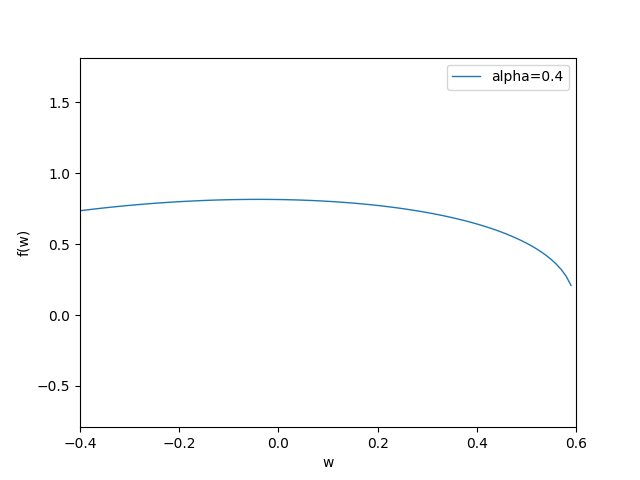
\includegraphics[width=50mm]{temp/0.4.png}
   \end{center}
   \caption{$\alpha=0.4$}
  \end{minipage}
  \begin{minipage}{0.33\hsize}
  \begin{center}
   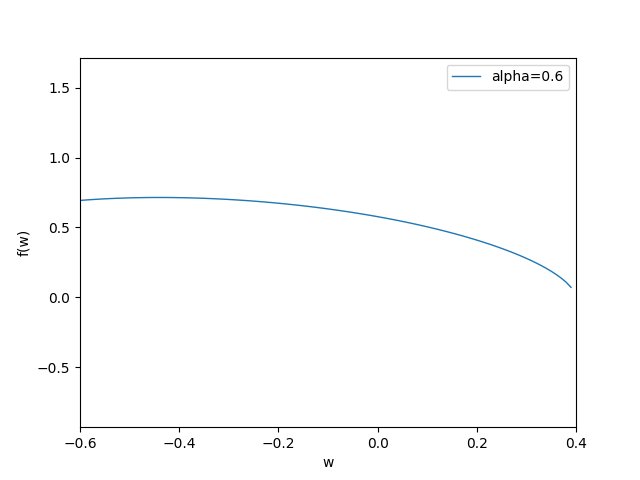
\includegraphics[width=50mm]{temp/0.6.png}
  \end{center}
   \caption{$\alpha=0.6$}
  \end{minipage}
  \begin{minipage}{0.33\hsize}
  \begin{center}
   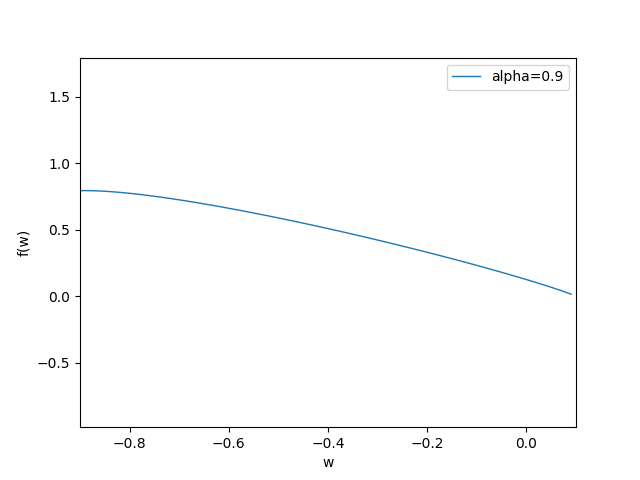
\includegraphics[width=50mm]{temp/0.9.png}
  \end{center}
   \caption{$\alpha=0.9$}
  \end{minipage}
 \end{figure}

\clearpage
\prb{II}{2}{A}{量子力学}
\begin{enumerate}
  \item 
  シュレーディンガー方程式を$-\varepsilon,+\varepsilon$で積分すると
  \begin{equation}
    -\frac{\hbar^2}{2m}\left[  
      \varphi'(\varepsilon)-\varphi'(-\varepsilon)
    \right]
    -
    \lambda\varphi(0)
    =
    E\int_{-\varepsilon}^{\varepsilon}\varphi(x)\dd x
  \end{equation}
  である.これの極限$\varepsilon\rightarrow0$をとれば
  \begin{equation}
    \lim_{\varepsilon\rightarrow+0}\left[  
      \varphi'(\varepsilon)-\varepsilon'(-\varepsilon)
    \right]
    =
    -\frac{2m\lambda}{\hbar^2}\varphi(0)
  \end{equation}
  である.

  \item
  シュレディンガー方程式は
  \begin{equation}
    \dv[2]{\varphi(x)}{x}
    +
    \frac{2m\lambda}{\hbar^2}\delta(x)\varphi(x)
    =
    \kappa^2\varphi(x)
  \end{equation}
  なので,解は
  \begin{equation}
    \varphi(x)
    =
    \begin{dcases}
      Ae^{+\kappa x}+Be^{-\kappa x}
      & 
      (x>0)
      \\
      Ce^{+\kappa x}+De^{-\kappa x}
      & 
      (x<0)
    \end{dcases}
  \end{equation}
  である.このとき,無限遠方で波動関数が0になっていることに気をつけ,係数を1とすれば
  \begin{equation}
    \varphi(x)
    =
    \begin{dcases}
      e^{-\kappa x}
      & 
      (x>0)
      \\
      e^{+\kappa x}
      & 
      (x<0)
    \end{dcases}
  \end{equation}
  である.

  \item 
  式(B)に素直に代入すれば
  \begin{equation}
    \kappa
    =
    \frac{m\lambda}{\hbar^2}
  \end{equation}
  である.

  \item 
  代入して
  \begin{equation}
    E
    =
    \frac{\hbar^2k^2}{2m}
  \end{equation}
  である.

  \item 
  連続性は
  \begin{equation}
    1+A=B
  \end{equation}
  で,傾きの関係(B)は
  \begin{equation}
    ik
    (1-A-B)
    =
    -\frac{2m\lambda}{\hbar^2}B
  \end{equation}
  なので,これらを連立して解けば
  \begin{equation}
    A
    =
    \frac{m\lambda}{i\hbar^2 k-m\lambda}
    \ ,\ \ 
    B
    =
    \frac{i\hbar^2 k}{i\hbar^2 k-m\lambda}
  \end{equation}
  である.

  \item 
  計算すれば
  \begin{equation}
    |A|^2
    =
    \frac{m^2\lambda^2}{\hbar^4 k^2+m^2\lambda^2}
    \ ,\ \ 
    |B|^2
    =
    \frac{\hbar^4 k^2}{\hbar^4 k^2+m^2\lambda^2}
  \end{equation}
  である.

\end{enumerate}

\clearpage
\prb{II}{2}{C}{力学}
\begin{enumerate}
  \item 
  それぞれ
  \begin{equation}
    \begin{dcases}
      T
      &=
      \frac{1}{2}ml^2\dot{\theta}_{1}^2
      +
      \frac{1}{2}ml^2\dot{\theta}_{2}^2
      \\
      U
      &=
      \frac{1}{2}mgl\theta_{1}^2
      +
      \frac{1}{2}mgl\theta_{2}^2
      +
      \frac{1}{2}k(\theta_{1}-\theta_{2})^2
    \end{dcases}
  \end{equation}
  である.

  \item 
  $\theta_{1},\theta_{2}$におけるオイラー・ラグランジュ方程式は
  \begin{equation}
    \begin{dcases}
      ml^2\ddot{\theta}_{1}
      +
      (mgl+k)\theta_{1}-k\theta_{2}
      &=
      0
      \\
      ml^2\ddot{\theta}_{2}
      +
      k\theta_{1}-(mgl+k)\theta_{2}
      &=
      0
    \end{dcases}
  \end{equation}
  なので,係数行列は
  \begin{equation}
    \begin{pmatrix}
      -g/l-k/ml^2 & k/ml^2 \\
      k/ml^2 & -g/l-k/ml^2
    \end{pmatrix}
  \end{equation}
  である.

  \item 
  微分方程式に,解を代入すれば
  \begin{equation}
    -\omega^2
    \begin{pmatrix}
      \theta_{1} \\
      \theta_{2}
    \end{pmatrix}
    =
    \begin{pmatrix}
      -g/l-k/ml^2 & k/ml^2 \\
      k/ml^2 & -g/l-k/ml^2
    \end{pmatrix}
    \begin{pmatrix}
      \theta_{1} \\
      \theta_{2}
    \end{pmatrix}
  \end{equation}
  である.よって,$-\omega^2$はこの係数行列の固有値になっているため,固有方程式を解けばよい.固有方程式は
  \begin{equation}
    \begin{vmatrix}
      \lambda+g/l+k/ml^2 & -k/ml^2 \\
      -k/ml^2 & \lambda+g/l+k/ml^2
    \end{vmatrix}
    =
    0
  \end{equation}
  なので,これを解けば
  \begin{equation}
    \lambda
    =
    -\frac{g}{l}
    \ ,\ \ 
    -\frac{g}{l}
    -\frac{2k}{ml^2}
  \end{equation}
  であり,
  \begin{equation}
    \omega_{-}
    =
    \sqrt{\frac{g}{l}}
    \ ,\ \ 
    \omega_{+}
    =
    \sqrt{\frac{g}{l}
    +\frac{2k}{ml^2}}
  \end{equation}
  である.

  \item 
  \uline{$\omega_{-}$のとき}

  固有ベクトルは$(1,1)$なので
  \begin{equation}
    Q_{1}=Q_{2}
    \ ,\ \ 
    \delta_{1}=\delta_{2}
  \end{equation}
  である.

  \uline{$\omega_{+}$のとき}

  固有ベクトルは$(1,-1)$なので
  \begin{equation}
    Q_{1}=Q_{2}
    \ ,\ \ 
    \delta_{1} -\delta_{2} = \pi
  \end{equation}
  である.
  
  この結果を踏まえれば,任意定数に位相をいれて
  \begin{equation}
    \begin{pmatrix}
      \theta_{1}(t) \\
      \theta_{2}(t)
    \end{pmatrix}
    =
    A
    \begin{pmatrix}
      1 \\
      1  
    \end{pmatrix}
    \sin \omega_{-}t
    +
    B
    \begin{pmatrix}
      1 \\
      -1
    \end{pmatrix}
    \sin \omega_{+}t
  \end{equation}
  である.

  \item 
  $t=0$で
  \begin{align}
    \dot{\theta}_{1}(0)
    =
    A\omega_{-}+B\omega_{+}
    &=
    \Omega_{0}
    \\
    \dot{\theta}_{2}(0)
    =
    A\omega_{-}-B\omega_{+}
    &=
    0
  \end{align}
  なので
  \begin{equation}
    A
    =
    \frac{\Omega_{0}}{2\omega_{-}}
    \ ,\ \ 
    B
    =
    \frac{\Omega_{0}}{2\omega_{+}}
  \end{equation}
  であり,
  \begin{align}
    \theta_{1}(t)
    &=    
    \frac{\Omega_{0}}{2\omega_{-}}
    \sin\omega_{-}t
    +    
    \frac{\Omega_{0}}{2\omega_{+}}
    \sin\omega_{+}t
    \\
    \theta_{2}(t)
    &=
    \frac{\Omega_{0}}{2\omega_{-}}
    \sin\omega_{-}t
    -
    \frac{\Omega_{0}}{2\omega_{+}}
    \sin\omega_{+}t
  \end{align}
  である.また,$\omega_{+}\sim\omega_{-}$とすると,$\theta_{2}$はそれぞれの項が打ち消しあって振動しなくなり,逆に$\theta_{1}$の振動がそろい振幅が大きくなる.

\end{enumerate}

\end{document}
